\IEEEPARstart{E}{n} este apartado, nos centramos a corroborar que los pasos de la implementaci\'on se dieron acorde a lo que cada m\'etodo visto propone. Para ello, creamos dos instancias en la cual se podr\'an visualizar con facilidad los cambios generados al aplicar el efecto de slowmotion. De hecho, uno de ellos se basar\'a de reproducir una sola im\'agen durante todo el video. El restante se basar\'a en observar el cambio entre los dos extremos que proporciona la escala de grises, es decir, de blanco a negro.
%---------------------------------------------------------------
\subsubsection{Blanco-Negro}

Nos situamos primero en el caso donde dicho video se comprende de dos tipos de frames, que es repetido una cierta cantidad de veces en un determinado tiempo. La particularidad de dichos frames, es que si se contempla \'estos como matriz, se confirma la igualdad en cada posici\'on del cuadro. Debido a que estamos trabajando sobre escala de grises, decidimos clasificar al tipo $A$ como un frame con todos sus p\'ixeles en negro (equivalente a $0$) y el tipo $B$ con p\'ixeles en blanco (equivalente a $255$).

En primer lugar, se seleccion\'o una im\'agen de esta caracter\'istica ya que nos podemos abstraer del procedimiento sobre el frame en conjunto. De esa manera, nos podemos enfocar en analizar cualquier posici\'on $(i,j)$. ¿Qu\'e utilidad nos brinda esto \'ultimo? El hecho de poder evaluar en detalle, el comportamiento del m\'etodo aferrado a nuestra implementaci\'on.

En segundo lugar, haber escogido dos valores que representan los extremos en la escala de representaci\'on, nos trae una mejor intuici\'on del resultado esperado. Con esto nos adelantamos a decir, que el video alentizado intentar\'a reflejar lo que sucede cuando se translada del tipo $A$ al $B$ mediante los frames interpolados.

Por \'ultimo, aclaramos que el video solo contendr\'a un cambio del frame de tipo $A$ al $B$, y ese mismo ser\'a definitorio.

\subsubsection*{Vecino m\'as cercano:}

Sabemos que su idea revoca en crear los cuadros intermedios copiando de un extremo u otro, tal como se explic\'o durante el desarrollo. Por ende, el resultado que \'este dar\'a al aplicarlo sobre el video, ser\'a bastante trivial. De hecho, lo \'unico que se podr\'a apreciar es la mayor duraci\'on del video resultante con respecto al original.

Pasamos a los resultados, que por la poca complejidad algor\'itmica que este m\'etodo implica, se validar\'a en brevedad a lo que se buscaba. 

\subsubsection*{\bf{Resultado:}}

Comprobamos que al decifrar los frames intermedios como matrices, \'estos se identificaron con su extremo m\'as cercano. Si al par\'ametro de cantidad de frames a adherir se le asignaba un n\'umero impar, luego en teor\'ia el valor del extremo derecho (en este caso, el blanco) tendr\'ia mayor presencia. Sin embargo, como la diferencia es de un solo frame adicional, no se not\'o nada en la pr\'actica debido a la cantidad de frames por segundo que corre el reproductor de video. 

En consecuencia, recolectamos la totalidad de frames del video en $slowmotion$ para comprobar si la implementaci\'on acert\'o con la distribuci\'on de cuadros intermedios.

\subsubsection*{Interpolaci\'on lineal:}

Nos inclinamos a una perspectiva que abarca mayor seriedad, ya que su comprobaci\'on se justificar\'a del lado matem\'atico. Si los u\'nicos dos puntos a trazar son el $(x0,y0) = (0,0)$ y $(x1,y1) = (1,255)$, luego la funci\'on a considerar tendr\'a la forma:

$f(x) = y0 + (y1-y0) * \frac{x - x0}{x1 - x0} = 255 * \frac{x}{255} = x$

Con esto \'ultimo, ya se puede considerar que tampoco traer\'a dificultad al momento de analizar correctitud.

\subsubsection*{\bf{Resultado:}}

Fuimos elevando el par\'ametro de entrada, agregando m\'as frames de por medio. De esta manera, el m\'etodo se encargaba de evaluar cada $f(x) = x$, con $x \in \{ \frac{1}{fr} ; \frac{2}{fr} \ldots ; \frac{fr}{fr} \}$. Como dicha funci\'on es creciente, notamos como efectivamente el avanze del video reflejaba el esclarecimiento del mismo, tomando valores de grises m\'as suaves hasta llegar al cero.

En este caso, mostramos un caso donde se le adicion\'o 10 frames, y luego comprobando al obtener la totalidad de im\'agenes, se verific\'o que los valores de los p\'ixeles intermedios, coincid\'ian con la funci\'on lineal en dicho punto. ( Ver figura \ref{fig:linealValidacion} ).


\begin{figure}[h!]
  \centering
    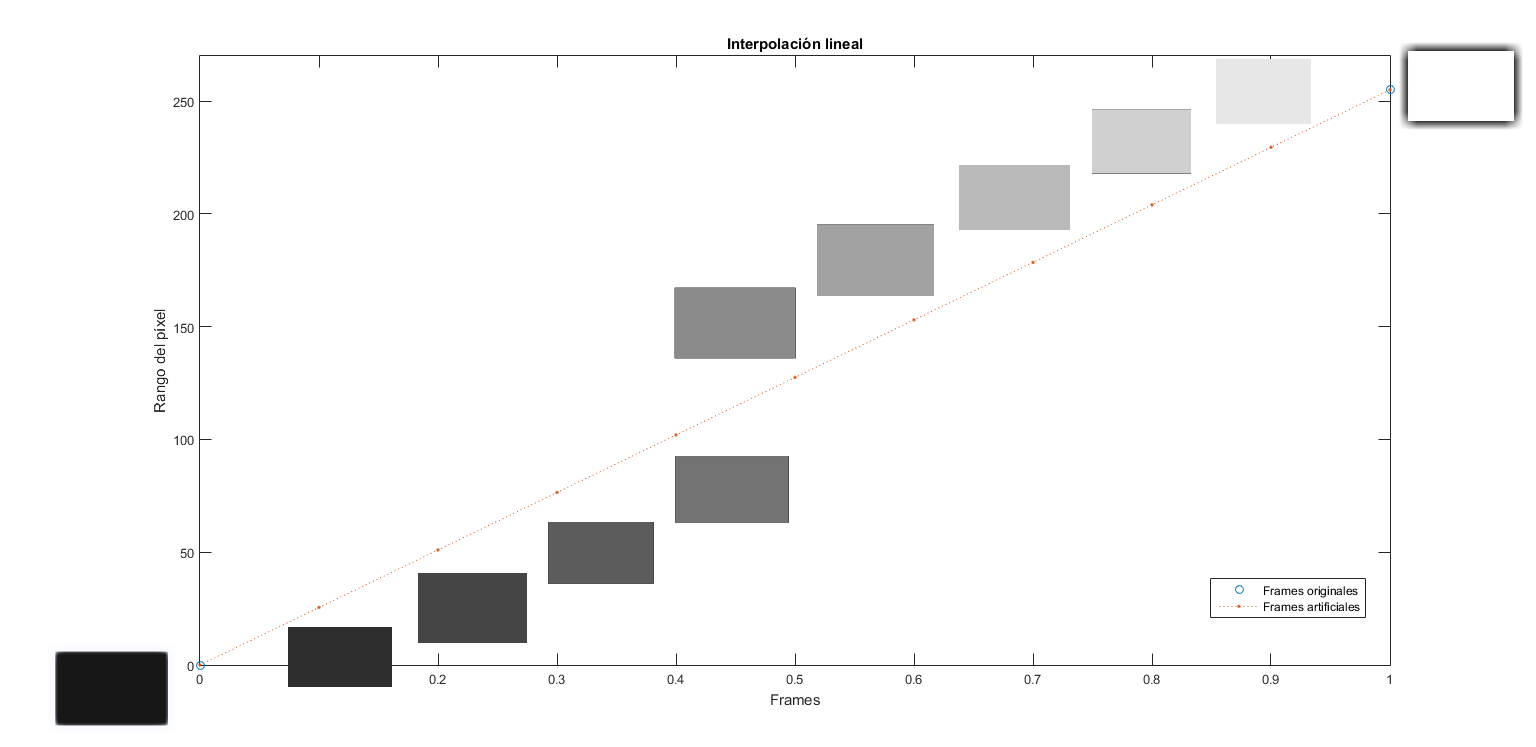
\includegraphics[width=0.75\textwidth]{GraficoLineal.png}
     \caption{Muestra del momento en que se realiza el cambio de blanco a negro, con sus respectivos frames intermedios}\label{fig:linealValidacion}
\end{figure}
\noindent

\subsubsection*{Splines}

Seguimos con la misma metodolog\'ia que con interpolaci\'on lineal, definiendo la funci\'on en cuesti\'on:

$f(x) = a (x - x0)^3 + b ( x - x0)^2 + c ( x - x0) + d$

Pero, ¿C\'omo hallamos los coeficientes del polinomio? Podr\'iamos por un lado, realizar las cuentas a papel y  de ah\'i seguir con el procedimiento de verificar con respecto a la implementaci\'on. Sin embargo, eso ser\'ia  bastante engorroso de realizar, por lo que optamos por usar un software inteligente cuyo nombre es $MatLab$. Usando la funci\'on $interpo1$ podemos obtener el valor de cualquier punto intermedio, en particular los que se evaluaron en nuestro programa.

No obstante, si bien al notar que efectivamente la funci\'on $f(x)$ se asemeja a una funci\'o lineal, hay que tener en cuenta una herramienta clave en $Splines$: la construcci\'on por bloques. Pero como decidimos que cada bloque comparta su primer y \'ultimo frame (excepto los extremos, que comparten alguno de los 2), luego no existe el caso de que se divida de forma tal que quede todo negro de un lado y blanco en lo que sigue.

\subsubsection*{\bf{Resultado:}}

Ideamos una instancia con par\'ametro de adici\'on de frames igual a 5, y dividido en 16 bloques. Como lo que importa aqu\'i es validaci\'on y no performance, optamos por un valor menor. Dicho esto, mediante $MatLab$ visualizamos cada Spline generado por bloque y comparando con la implementaci\'on, no se encontr\'o ninguna objeci\'on a lo ya comentado.

Con el gr\'afico \ref{fig:splineValidacion}, identificamos lo que $MatLab$ produjo al enviarle los puntos pertenecientes al bloque donde se hallaba el cambio de blanco a negro y de ah\'i, comparamos con los frames que obtuvimos.

\begin{figure}[h!]
  \centering
    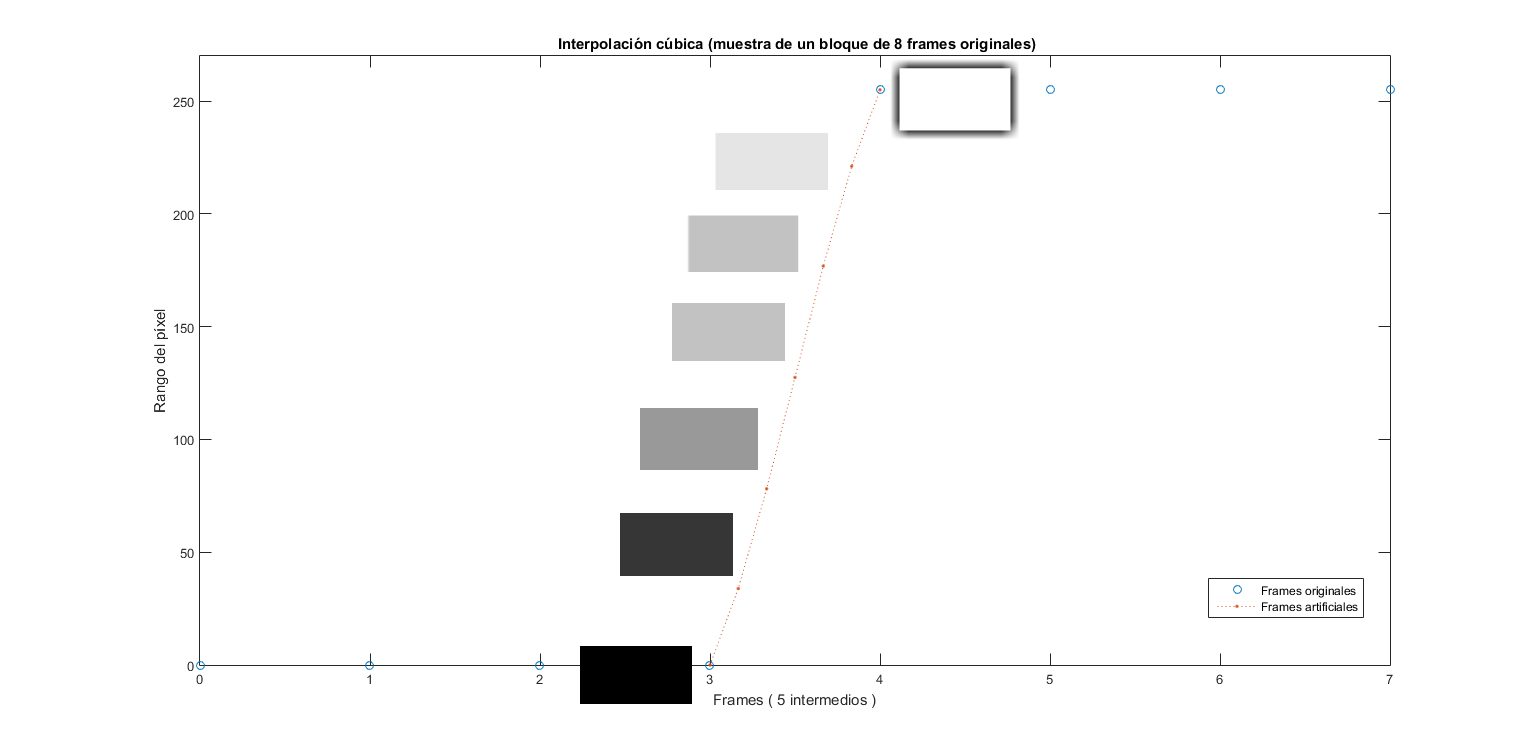
\includegraphics[width=0.75\textwidth]{GraficoSplines.png}
     \caption{Muestra del bloque que contiene el cambio, con los cuadros comparados}\label{fig:splineValidacion}
\end{figure}
\noindent

%---------------------------------------------------------------
\subsubsection{C\'amara Fija - Im\'agen Fija}

Equivalente a pensar que una im\'agen est\'a siendo reproducida durante un lapso de tiempo, que difiere al hecho de que una c\'amara est\'e quieta, enfocando a un objeto que puede ser sofocado por la luz. Y est\'a claro que el mero hecho de querer alentizar un video de tal caracter\'istica, solo servir\'a para aumentar la duraci\'on de la misma. Por lo conceptualmente visto, no hay dudas de que si la implementaci\'on se realiz\'o de forma correcta, no existir\'ia ning\'un cambio en el video.

Usamos metodolog\'ias id\'enticas para los tres m\'etodos. Esto es, extraer cada cuadro artificial y corroborar que coincide con la foto utilizada.

\subsubsection*{\bf{Resultado:}}

Como en cada p\'ixel $(i,j)$ el valor se mantuvo constante, as\'i lo fue con las funciones interpoladoras. De esta manera, cualquier punto que era evaluado por m\'as frames que se le quisiese acomodar, solo produc\'ia un video m\'as largo. En conclusi\'on, la im\'agen permeneci\'o intacta durante toda su reproducci\'on.
